\documentclass[11pt,a4paper]{article}

\usepackage[
  top=0.72in,
  bottom=0.78in,
  left=0.62in,
  right=0.62in,
]{geometry}

\usepackage{microtype}
\usepackage{graphicx}
\usepackage{booktabs}
\usepackage{tabularx}
\usepackage{array}
\usepackage{adjustbox}
\usepackage{amsmath,amssymb}
\usepackage{caption}
\usepackage{float}
\usepackage{placeins}
\usepackage{flafter}
\usepackage{dblfloatfix}
\usepackage{tikz}
\usepackage{pgfplots}
\pgfplotsset{
  compat=1.18,
  tick label style={font=\footnotesize},
  label style={font=\footnotesize},
  legend style={font=\footnotesize},
}
\usetikzlibrary{positioning,arrows.meta}

\usepackage[numbers,sort&compress]{natbib}
\usepackage{hyperref}
\hypersetup{colorlinks=true, linkcolor=blue, citecolor=blue, urlcolor=blue}

\captionsetup{font=small, labelfont=bf, skip=6pt, justification=raggedright}
\captionsetup[table]{position=above, skip=8pt}
\emergencystretch=2em

\newcommand{\tablestarfit}[1]{%
  \centering\adjustbox{max width=\textwidth,center}{#1}%
}

% Qualitative: fixed-width 3-column grid (full figure* width)
\newlength{\qualimgw}
\setlength{\qualimgw}{0.30\linewidth}

\newcommand{\qualrowheader}[2]{%
  \par\vspace{0.35em}%
  \noindent\centering\textbf{#1}: \textit{#2}\par\vspace{0.25em}%
}

\newcommand{\qualpanelrow}[9]{%
  \centering
  \begin{tabular}{@{}c@{\hspace{0.025\linewidth}}c@{\hspace{0.025\linewidth}}c@{}}
    \includegraphics[width=\qualimgw]{#1} &
    \includegraphics[width=\qualimgw]{#2} &
    \includegraphics[width=\qualimgw]{#3} \\[0.35em]
    \parbox[t]{\qualimgw}{\centering\footnotesize\textbf{#4}\\[0.15em]\footnotesize #5} &
    \parbox[t]{\qualimgw}{\centering\footnotesize\textbf{#6}\\[0.15em]\footnotesize #7} &
    \parbox[t]{\qualimgw}{\centering\footnotesize\textbf{#8}\\[0.15em]\footnotesize #9} \\
  \end{tabular}\par\vspace{0.2em}%
}


\title{\textbf{Locate-SAM2: LocateAnything-Guided SAM2}\\[0.2em]
  \large A Training-Free Study of Zero-Shot Referring-Expression Segmentation}

% Edit author block here (single source for title page)
\newcommand{\PaperAuthorName}{Jerardh Josekutty}
\newcommand{\PaperAuthorAffiliation}{Affiliation TBD}
\newcommand{\PaperAuthorEmail}{email@domain.edu}
\newcommand{\PaperAuthorUrl}{}

\author{%
  \textbf{\PaperAuthorName}\\[0.2em]
  \normalsize \PaperAuthorAffiliation\\[0.15em]
  \texttt{\PaperAuthorEmail}\\[0.2em]
  \footnotesize Code: \texttt{URL to be added before public release}%
}

\date{\today}

\begin{document}
\maketitle

\begin{abstract}
\noindent
Referring-expression segmentation needs two decisions: which object a phrase denotes, and which pixels belong to that object.
Promptable segmenters such as SAM~2.1 solve the second part well when given a good box, but they do not ground language by themselves.
We study whether \textbf{LocateAnything-3B}, a parallel-box vision-language grounder, is a stronger front end than Grounding DINO for a frozen Grounded-SAM-style pipeline.
\textbf{Locate-SAM2} keeps all components fixed: LocateAnything predicts boxes, a small Prompt-to-Mask Adapter converts boxes into SAM prompts, and SAM~2.1 returns the final mask.
We evaluate the same frozen system on the three standard RefCOCO-family validation splits.
Locate-SAM2 hybrid reaches \textbf{0.772} mIoU on RefCOCO, \textbf{0.717} on RefCOCO+, and \textbf{0.746} on RefCOCO-g.
Against DINO-Base + SAM2 under the same adapter, the gains are \textbf{+5.5}, \textbf{+10.5}, and \textbf{+8.0} mIoU; against DINO-Tiny + SAM2, the gains are \textbf{+33.1}, \textbf{+27.7}, and \textbf{+24.3} mIoU.
On RefCOCO testA/testB, hybrid reaches \textbf{0.807}/\textbf{0.730} mIoU versus \textbf{0.761}/\textbf{0.661} for DINO-Base; on RefCOCO+ testA/testB, it reaches \textbf{0.766}/\textbf{0.650} versus \textbf{0.708}/\textbf{0.517}.
GT-box + SAM2 oracles reach \textbf{0.836}, \textbf{0.836}, and \textbf{0.815} mIoU, so hybrid recovers \textbf{85.8--92.3\%} of the oracle result depending on split.
The main finding is that better language-conditioned boxes consistently improve zero-shot text-to-mask segmentation, while the remaining errors are mostly wrong-object grounding rather than SAM boundary failures.
The tradeoff is higher latency and memory.
\end{abstract}
\vspace{0.75em}

%==============================================================================
\section{Introduction}
\label{sec:intro}

Referring expression segmentation (RES) asks for the pixel mask of the object denoted by a text phrase, such as ``the red cup behind the laptop.''
Promptable segmenters such as SAM and SAM~2~\cite{kirillov2023sam,ravi2024sam2} can produce high-quality masks from boxes, points, or masks, but they do not decide \emph{which} object a phrase refers to.
Grounded SAM-style systems~\cite{ren2024groundedsam} solve this by pairing an open-vocabulary \emph{grounder}, commonly Grounding DINO~\cite{liu2023groundingdino}, with SAM:
\begin{center}
\small \texttt{text $\rightarrow$ box $\rightarrow$ mask}.
\end{center}

\textbf{LocateAnything}~\cite{wang2026locateanything} introduces parallel box decoding for visual grounding.
We ask:
\emph{Can LocateAnything serve as a drop-in grounder for a Grounded-SAM-style RES pipeline, and where does the resulting system fail?}

\textbf{Locate-SAM2} uses a fixed, training-free assembly:
LocateAnything-3B $\rightarrow$ Prompt-to-Mask Adapter $\rightarrow$ SAM~2.1 (\texttt{sam2.1-hiera-large}).
The paper is built on these two existing model families.
We do not modify LocateAnything or SAM2; our work is the pipeline integration, adapter design choices, matched evaluation, and error analysis.
By keeping SAM and the adapter fixed across methods, the evaluation isolates the value and limits of the grounding stage.

\paragraph{Contributions.}
\begin{enumerate}
  \item A reproducible LocateAnything $\rightarrow$ SAM~2.1 pipeline and evaluation harness for zero-shot RES, without training either model.
  \item Full RefCOCO, RefCOCO+, and RefCOCO-g validation against DINO-Tiny, DINO-Base, and GT-box + SAM2 oracles.
  \item Adapter ablations showing that box prompts are the main usable interface to SAM in this setting; point-only prompting falls to $\sim$0.51 mIoU.
  \item Qualitative and oracle analysis showing that SAM usually segments the selected box well, so wrong-instance errors are primarily grounding errors.
\end{enumerate}

\paragraph{Scope.}
This is a \textbf{systems and evaluation} paper, not a supervised RES benchmark-leader claim.
Locate-SAM2 is best read as a zero-shot mask proposal pipeline for research datasets, annotation workflows, and settings where target categories are not fixed in advance.

%==============================================================================
\section{Related Work}
\label{sec:related}

\paragraph{Grounded SAM-style pipelines.}
Modular open-vocabulary segmentation systems combine a language-conditioned detector or grounder with SAM~\cite{ren2024groundedsam}.
Our evaluation follows this recipe while keeping SAM~2.1 and the adapter settings fixed across methods.

\paragraph{Grounding DINO.}
Grounding DINO~\cite{liu2023groundingdino} is the standard open-vocabulary detector baseline for this modular family.
We evaluate Tiny and Base checkpoints with the same SAM2 backend and adapter.
DINO-Base is the primary baseline; DINO-Tiny is included as a lower-compute reference commonly used in Grounded-SAM-style examples.

\paragraph{LocateAnything.}
LocateAnything~\cite{wang2026locateanything} is the core grounder in this paper.
It replaces sequential coordinate-token generation with Parallel Box Decoding, where boxes and points are decoded as structured units rather than independent coordinate tokens.
The original NVIDIA report evaluates it for grounding and detection; we test whether its boxes improve a SAM2-based text-to-mask pipeline.
This is a use of LocateAnything, not a replacement for the LocateAnything method itself.

\paragraph{Referring expression segmentation.}
Classic referring expression work studies how language identifies an image region or mask, from modular comprehension models such as MAttNet~\cite{yu2018mattnet} to mask-producing RES systems such as CRIS~\cite{wang2022cris} and LAVT~\cite{yang2022lavt}.
Recent supervised or large-scale trained systems, including UniRES++~\cite{liu2025unirespp}, report leading results on RefCOCO-family benchmarks.
Generalized RES systems such as GRES~\cite{liu2023gres} and CoHD~\cite{luo2025cohd} further study multiple-referent and no-target settings.
These papers define the task family and motivate careful evaluation, but they are a different regime from Locate-SAM2: they train or adapt models for RES masks, while we evaluate a frozen modular pipeline.
We therefore compare only modular zero-shot pipelines and use the GT-box oracle to separate grounding quality from mask quality.

\paragraph{Native text-prompted segmentation.}
SAM~3~\cite{sam3_2025} supports concept prompts for detecting, segmenting, and tracking matching objects.
Locate-SAM2 instead studies a modular setting where the grounder and segmenter remain separate, so the grounding stage can be swapped, timed, and compared directly.

%==============================================================================
\section{Method}
\label{sec:method}

Given image $I$ and referring expression $q$, Locate-SAM2 executes three stages:
\textbf{(1)~Grounding:} LocateAnything-3B predicts one or more axis-aligned boxes for $q$.
\textbf{(2)~Prompt-to-Mask Adapter:} the system validates boxes, optionally crops around each candidate, forms SAM prompts, and reranks masks.
\textbf{(3)~Segmentation:} SAM~2.1 outputs the final mask $\hat{M}$.
No component is finetuned.

\begin{figure}[t]
  \centering
  \begin{adjustbox}{max width=\textwidth}
  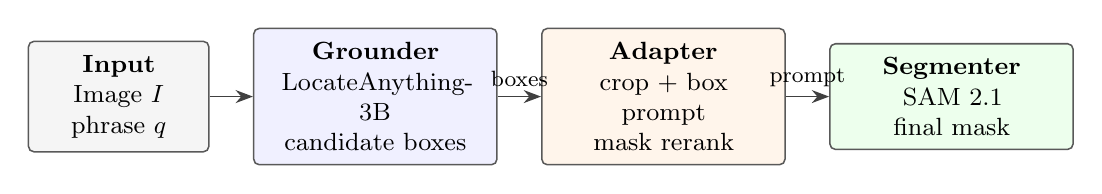
\begin{tikzpicture}[
    font=\small,
    stage/.style={draw=black!65, line width=0.55pt, rounded corners=2pt,
      align=center, text width=0.22\textwidth, minimum height=1.08cm,
      inner xsep=6pt, inner ysep=5pt},
    io/.style={draw=black!65, line width=0.55pt, rounded corners=2pt,
      align=center, text width=0.16\textwidth, minimum height=1.08cm,
      inner xsep=5pt, inner ysep=5pt},
    arr/.style={-{Stealth[length=2.2mm]}, line width=0.65pt, draw=black!75},
  ]
    \node[io, fill=gray!8] (input) {\textbf{Input}\\Image $I$\\phrase $q$};
    \node[stage, fill=blue!6, right=0.55cm of input] (ground) {\textbf{Grounder}\\LocateAnything-3B\\candidate boxes};
    \node[stage, fill=orange!8, right=0.55cm of ground] (adapter) {\textbf{Adapter}\\crop + box prompt\\mask rerank};
    \node[stage, fill=green!7, right=0.55cm of adapter] (sam) {\textbf{Segmenter}\\SAM~2.1\\final mask};
    \draw[arr] (input) -- (ground);
    \draw[arr] (ground) -- node[above, font=\footnotesize] {boxes} (adapter);
    \draw[arr] (adapter) -- node[above, font=\footnotesize] {prompt} (sam);
  \end{tikzpicture}
  \end{adjustbox}
  \caption{%
    \textbf{Locate-SAM2 evaluation pipeline.}
    LocateAnything-3B supplies boxes, the adapter converts boxes into SAM2 prompts, and SAM~2.1 produces the mask.
    Baselines replace LocateAnything with Grounding DINO Tiny or Base; the oracle replaces the predicted box with the RefCOCO ground-truth box.
    SAM~2.1 and the adapter settings are fixed across non-oracle methods.}
  \label{fig:arch}
\end{figure}

\subsection{Prompt-to-Mask Adapter}
\label{sec:adapter}

The adapter is deliberately small.
It validates the grounder's box, expands the box by 5\% before cropping so SAM sees local context, and passes the box to SAM~2.1 as the main prompt.
The default configuration is \texttt{box} prompting, \texttt{crop} mode, and \texttt{best\_score} mask selection.
When SAM2 returns multiple mask candidates (\texttt{multimask\_output=true}), \texttt{best\_score} selects the mask with the highest SAM predicted mask IoU from \texttt{iou\_scores}.
We also ablate \texttt{box\_point} and \texttt{point} prompts, full-image inference without cropping, \texttt{top1} reranking, and LocateAnything \texttt{fast} versus \texttt{hybrid} generation.

%==============================================================================
\section{Experimental Setup}
\label{sec:experiments}

\paragraph{Datasets.}
We evaluate RefCOCO val ($n{=}3{,}811$), RefCOCO+ val ($n{=}3{,}805$), and RefCOCO-g val ($n{=}5{,}000$, Google split)~\cite{kazemzadeh2014refcoco,yu2016refcoco} using COCO \texttt{train2014} images and masks from the split annotations.
We also report RefCOCO and RefCOCO+ testA/testB splits for the primary DINO-Base comparison.

\paragraph{Metrics.}
We report mean mask IoU, cumulative IoU (cIoU), precision at IoU thresholds from 0.5 to 0.9, mean box IoU, latency split by grounding and SAM, and peak VRAM.

\paragraph{Protocol.}
All full-validation numbers use seed 42 and the shared adapter configuration (\texttt{box}, \texttt{crop}, \texttt{best\_score}) unless explicitly ablated.
DINO-Tiny uses box/text thresholds 0.25/0.25 after a 200-ref threshold sweep; several settings tie near 0.426 mIoU.
Numbers are read from \texttt{outputs/full\_val/}, \texttt{outputs/refcoco\_plus/}, and \texttt{outputs/refcocog/}.
Experiments were run on a single NVIDIA RTX PRO 6000 Blackwell GPU with 96\,GB VRAM.
Latency is wall-clock inference time averaged over the split on this hardware, and VRAM is peak allocated memory during inference.
The peak-memory gap is a practical deployment constraint: hybrid uses about 8.9\,GB versus about 3.1\,GB for DINO-Base.

%==============================================================================
\section{Results and Analysis}
\label{sec:results}

\subsection{Main quantitative results}
\label{sec:main-results}

Table~\ref{tab:main} reports RefCOCO val; Table~\ref{tab:refcoco-plus} reports RefCOCO+; Table~\ref{tab:refcocog} reports RefCOCO-g (Google split, $n{=}5{,}000$); Table~\ref{tab:test-splits} reports testA/testB.
The results answer the main question of the paper: replacing Grounding DINO with LocateAnything improves the zero-shot text-to-mask pipeline under the same SAM2 backend and adapter.
On RefCOCO, Locate-SAM2 hybrid is \textbf{+33.1} mIoU over DINO-Tiny and \textbf{+5.5} mIoU over DINO-Base.
On RefCOCO+, hybrid is \textbf{+27.7} mIoU over DINO-Tiny and \textbf{+10.5} mIoU over DINO-Base.
On RefCOCO-g, hybrid is \textbf{+24.3} mIoU over DINO-Tiny and \textbf{+8.0} mIoU over DINO-Base.
Fast mode is close to hybrid on all three splits and is especially close on RefCOCO+ (0.709 vs.\ 0.717 mIoU), but hybrid is the best non-oracle setting in every table.
The improvement comes with a practical cost: LocateAnything-3B uses more memory and latency than DINO-Base in this setup.

\paragraph{Interpretation.}
Within this controlled frozen pipeline, the grounder changes final mask quality by a large margin.
The test splits show the same pattern as validation: hybrid beats DINO-Base on all four RefCOCO/RefCOCO+ test splits, with gains from +4.6 to +13.3 mIoU.
This result should not be read as a supervised RES leaderboard claim; it is evidence that stronger language-conditioned boxes matter when SAM is held fixed.

% Result tables in one consistent typography block.

\begin{table}[t]
  \centering
  \caption{RefCOCO val ($n{=}3{,}811$, seed 42). Best non-oracle in \textbf{bold}.}
  \label{tab:main}
  \footnotesize
  \setlength{\tabcolsep}{4.8pt}
  \begin{tabular*}{\textwidth}{@{\extracolsep{\fill}}lccccccc@{}}
    \toprule
    Method & mIoU & cIoU & P@0.5 & P@0.7 & Box IoU & ms & GB \\
    \midrule
    DINO-Tiny + SAM2    & 0.441 & 0.354 & 48.6 & 43.3 & 0.506 & 146 & 2.9 \\
    DINO-Base + SAM2    & 0.717 & 0.657 & 81.7 & 74.4 & 0.802 & 164 & 3.1 \\
    Locate-SAM2 fast    & 0.769 & 0.745 & 87.5 & 79.2 & 0.847 & 190 & 8.9 \\
    \textbf{Locate-SAM2 hybrid} & \textbf{0.772} & \textbf{0.753} & \textbf{88.1} & \textbf{80.0} & \textbf{0.851} & \textbf{195} & \textbf{8.9} \\
    GT-box + SAM2 oracle & 0.836 & 0.830 & 95.2 & 88.5 & 1.000 & 72  & 1.3 \\
    \bottomrule
  \end{tabular*}

  \vspace{0.7em}

  \begin{minipage}[t]{0.47\textwidth}
    \centering
    \captionof{table}{RefCOCO+ val ($n{=}3{,}805$).}
    \label{tab:refcoco-plus}
    \scriptsize
    \renewcommand{\arraystretch}{1.08}
    \setlength{\tabcolsep}{3pt}
    \begin{tabular*}{\linewidth}{@{\extracolsep{\fill}}lcccc@{}}
      \toprule
      Method & mIoU & P@0.5 & Box IoU & ms \\
      \midrule
      DINO-Tiny + SAM2  & 0.440 & 47.7 & 0.502 & 146 \\
      DINO-Base + SAM2  & 0.612 & 69.4 & 0.691 & 164 \\
      Locate-SAM2 fast  & 0.709 & 80.3 & 0.784 & 188 \\
      \textbf{Locate-SAM2 hybrid} & \textbf{0.717} & \textbf{81.6} & \textbf{0.795} & 198 \\
      GT-box + SAM2 oracle & 0.836 & 95.2 & 1.000 & 72 \\
      \bottomrule
    \end{tabular*}
  \end{minipage}\hfill
  \begin{minipage}[t]{0.47\textwidth}
    \centering
    \captionof{table}{Adapter ablations (200 refs, seed 42).}
    \label{tab:ablation}
    \scriptsize
    \setlength{\tabcolsep}{3pt}
    \begin{tabular*}{\linewidth}{@{\extracolsep{\fill}}lcc@{}}
      \toprule
      Config & mIoU & P@0.5 \\
      \midrule
      default (hybrid, box, crop) & 0.777 & 89.5 \\
      box + point & 0.766 & 89.0 \\
      \textbf{point only} & \textbf{0.509} & \textbf{56.0} \\
      no crop & 0.784 & 89.5 \\
      top1 rerank & 0.775 & 89.5 \\
      \bottomrule
    \end{tabular*}
  \end{minipage}
\end{table}

\begin{table}[t]
  \centering
  \caption{RefCOCO-g val ($n{=}5{,}000$, Google split).}
  \label{tab:refcocog}
  \footnotesize
  \setlength{\tabcolsep}{4.8pt}
  \begin{tabular*}{\textwidth}{@{\extracolsep{\fill}}lccccccc@{}}
    \toprule
    Method & mIoU & cIoU & P@0.5 & P@0.7 & Box IoU & ms & GB \\
    \midrule
    DINO-Tiny + SAM2    & 0.503 & 0.414 & 55.7 & 49.1 & 0.588 & 148 & 2.9 \\
    DINO-Base + SAM2    & 0.666 & 0.589 & 75.4 & 67.5 & 0.760 & 166 & 3.1 \\
    Locate-SAM2 fast    & 0.741 & 0.719 & 84.0 & 74.3 & 0.835 & 199 & 8.9 \\
    \textbf{Locate-SAM2 hybrid} & \textbf{0.746} & \textbf{0.725} & \textbf{85.0} & \textbf{75.2} & \textbf{0.839} & \textbf{207} & \textbf{8.9} \\
    GT-box + SAM2 oracle & 0.815 & 0.815 & 93.1 & 84.6 & 1.000 & 72  & 1.3 \\
    \bottomrule
  \end{tabular*}
\end{table}

\begin{table}[t]
  \centering
  \caption{RefCOCO and RefCOCO+ test splits. Primary comparison is DINO-Base + SAM2 versus Locate-SAM2 hybrid under the same adapter.}
  \label{tab:test-splits}
  \footnotesize
  \setlength{\tabcolsep}{4.8pt}
  \begin{tabular*}{\textwidth}{@{\extracolsep{\fill}}llccccc@{}}
    \toprule
    Split & Method & $n$ & mIoU & P@0.5 & Box IoU & ms \\
    \midrule
    RefCOCO testA  & DINO-Base + SAM2 & 1,975 & 0.761 & 87.4 & 0.829 & 165 \\
    RefCOCO testA  & \textbf{Locate-SAM2 hybrid} & 1,975 & \textbf{0.807} & \textbf{93.1} & \textbf{0.868} & 192 \\
    RefCOCO testB  & DINO-Base + SAM2 & 1,810 & 0.661 & 73.5 & 0.757 & 164 \\
    RefCOCO testB  & \textbf{Locate-SAM2 hybrid} & 1,810 & \textbf{0.730} & \textbf{81.5} & \textbf{0.820} & 197 \\
    RefCOCO+ testA & DINO-Base + SAM2 & 1,975 & 0.708 & 81.3 & 0.774 & 165 \\
    RefCOCO+ testA & \textbf{Locate-SAM2 hybrid} & 1,975 & \textbf{0.766} & \textbf{88.2} & \textbf{0.828} & 194 \\
    RefCOCO+ testB & DINO-Base + SAM2 & 1,798 & 0.517 & 56.8 & 0.601 & 164 \\
    RefCOCO+ testB & \textbf{Locate-SAM2 hybrid} & 1,798 & \textbf{0.650} & \textbf{72.4} & \textbf{0.741} & 203 \\
    \bottomrule
  \end{tabular*}
\end{table}

\begin{figure*}[!t]
  \centering
  \small
  \begin{minipage}[t]{0.48\textwidth}
    \centering
    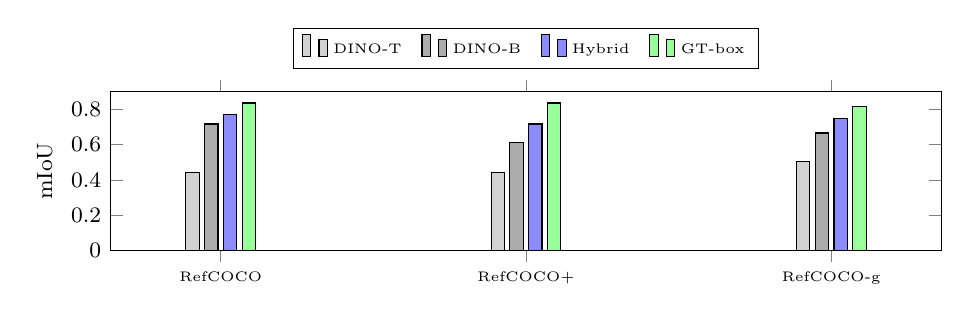
\begin{tikzpicture}
      \begin{axis}[
        width=\linewidth, height=3.6cm, ybar, bar width=4.8pt,
        ymin=0, ymax=0.90, ylabel={mIoU},
        symbolic x coords={RefCOCO,RefCOCO+,RefCOCO-g},
        xtick=data, xticklabel style={font=\tiny},
        enlarge x limits=0.18,
        legend style={
          font=\tiny,
          at={(0.5,1.14)},
          anchor=south,
          legend columns=4,
          /tikz/every even column/.append style={column sep=0.18cm}
        },
      ]
        \addplot[fill=gray!35] coordinates {(RefCOCO,0.441) (RefCOCO+,0.440) (RefCOCO-g,0.503)};
        \addplot[fill=gray!65] coordinates {(RefCOCO,0.717) (RefCOCO+,0.612) (RefCOCO-g,0.666)};
        \addplot[fill=blue!45] coordinates {(RefCOCO,0.772) (RefCOCO+,0.717) (RefCOCO-g,0.746)};
        \addplot[fill=green!40] coordinates {(RefCOCO,0.836) (RefCOCO+,0.836) (RefCOCO-g,0.815)};
        \legend{DINO-T,DINO-B,Hybrid,GT-box}
      \end{axis}
    \end{tikzpicture}
    \par\vspace{0.15em}(a) Main mIoU across validation splits
  \end{minipage}\hfill
  \begin{minipage}[t]{0.48\textwidth}
    \centering
    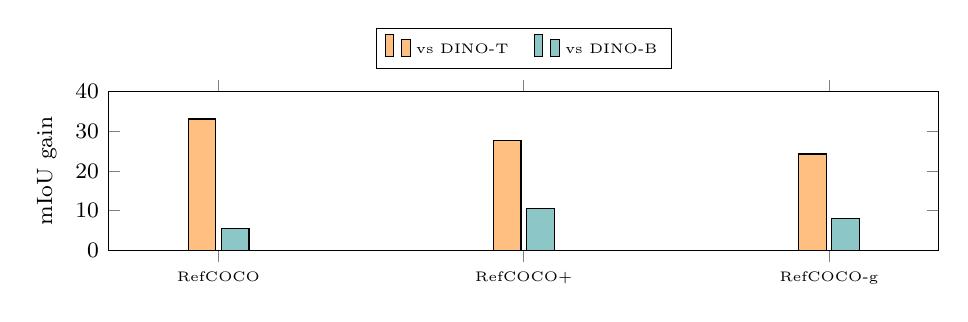
\begin{tikzpicture}
      \begin{axis}[
        width=\linewidth, height=3.6cm, ybar, bar width=10pt,
        ymin=0, ymax=40, ylabel={mIoU gain},
        symbolic x coords={RefCOCO,RefCOCO+,RefCOCO-g},
        xtick=data, xticklabel style={font=\tiny},
        enlarge x limits=0.18,
        legend style={
          font=\tiny,
          at={(0.5,1.14)},
          anchor=south,
          legend columns=2,
          /tikz/every even column/.append style={column sep=0.25cm}
        },
      ]
        \addplot[fill=orange!50] coordinates {(RefCOCO,33.1) (RefCOCO+,27.7) (RefCOCO-g,24.3)};
        \addplot[fill=teal!45] coordinates {(RefCOCO,5.5) (RefCOCO+,10.5) (RefCOCO-g,8.0)};
        \legend{vs DINO-T,vs DINO-B}
      \end{axis}
    \end{tikzpicture}
    \par\vspace{0.15em}(b) Hybrid gain over matched baselines
  \end{minipage}

  \vspace{0.55em}

  \begin{minipage}[t]{0.48\textwidth}
    \centering
    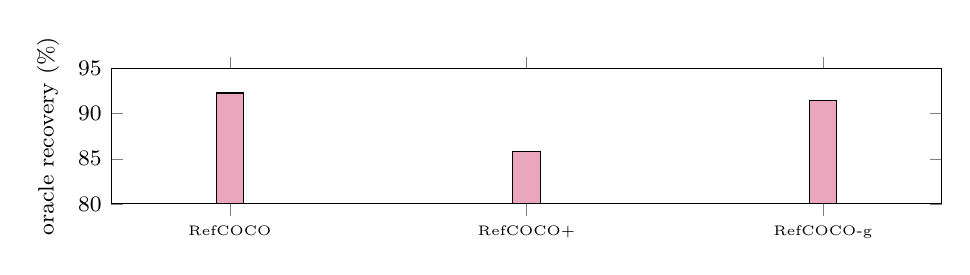
\begin{tikzpicture}
      \begin{axis}[
        width=\linewidth, height=3.3cm, ybar, bar width=10pt,
        ymin=80, ymax=95, ylabel={oracle recovery (\%)},
        symbolic x coords={RefCOCO,RefCOCO+,RefCOCO-g},
        xtick=data, xticklabel style={font=\tiny},
        enlarge x limits=0.2,
      ]
        \addplot[fill=purple!35] coordinates {(RefCOCO,92.3) (RefCOCO+,85.8) (RefCOCO-g,91.5)};
      \end{axis}
    \end{tikzpicture}
    \par\vspace{0.15em}(c) Hybrid as a percentage of GT-box oracle
  \end{minipage}\hfill
  \begin{minipage}[t]{0.48\textwidth}
    \centering
    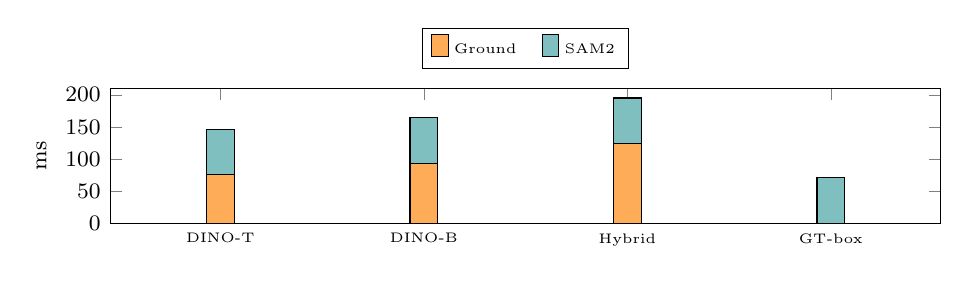
\begin{tikzpicture}
      \begin{axis}[
        width=\linewidth, height=3.3cm, ybar stacked, bar width=10pt,
        ymin=0, ymax=210, ylabel={ms},
        symbolic x coords={DINO-T,DINO-B,Hybrid,GT-box},
        xtick=data, xticklabel style={font=\tiny},
        legend style={
          font=\tiny,
          at={(0.5,1.14)},
          anchor=south,
          legend columns=2,
          /tikz/every even column/.append style={column sep=0.25cm}
        },
        enlarge x limits=0.18,
      ]
        \addplot[fill=orange!65] coordinates {(DINO-T,76) (DINO-B,94) (Hybrid,124) (GT-box,0)};
        \addplot[fill=teal!50] coordinates {(DINO-T,70) (DINO-B,71) (Hybrid,71) (GT-box,72)};
        \legend{Ground, SAM2}
      \end{axis}
    \end{tikzpicture}
    \par\vspace{0.15em}(d) RefCOCO latency breakdown
  \end{minipage}

  \vspace{0.55em}

  \begin{minipage}[t]{0.55\textwidth}
    \centering
    \begin{adjustbox}{max width=\linewidth}
    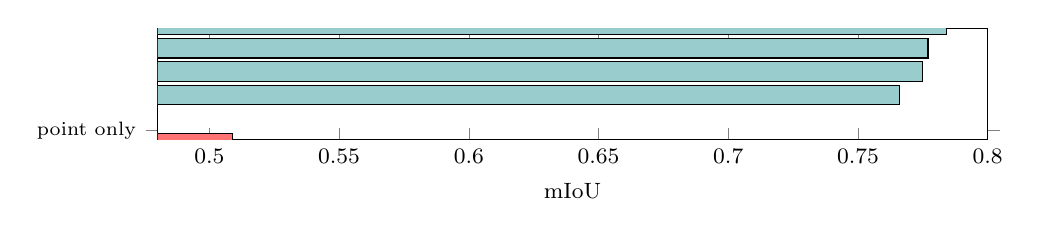
\begin{tikzpicture}
      \begin{axis}[
        width=\linewidth, height=3.0cm, xbar, bar width=7pt,
        xmin=0.48, xmax=0.80, xlabel={mIoU},
        symbolic y coords={point,boxpt,top1,default,full},
        yticklabels={point only, box+point, top1, default, no crop},
        ytick=data, yticklabel style={font=\scriptsize}, enlarge y limits=0.1,
      ]
        \addplot[fill=red!55] coordinates {(0.509,point)};
        \addplot[fill=teal!40] coordinates {(0.766,boxpt) (0.775,top1) (0.777,default) (0.784,full)};
      \end{axis}
    \end{tikzpicture}
    \end{adjustbox}
    \par\vspace{0.15em}(e) Adapter ablations
  \end{minipage}
  \caption{%
    \textbf{Quantitative summary.}
    (a) Hybrid is the best non-oracle method on RefCOCO, RefCOCO+, and RefCOCO-g.
    (b) Gains hold against both Grounding DINO baselines on every split.
    (c) Hybrid recovers 85.8--92.3\% of the GT-box oracle.
    (d) LocateAnything adds latency in exchange for stronger boxes.
    (e) Point-only prompting drops to $\sim$0.51 mIoU.}
  \label{fig:results-panel}
\end{figure*}


\subsection{Oracle diagnostic: grounding vs. mask quality}
\label{sec:oracle}

The GT-box oracle reaches 0.836 mIoU on RefCOCO, 0.836 on RefCOCO+, and 0.815 on RefCOCO-g.
Locate-SAM2 hybrid recovers 92.3\%, 85.8\%, and 91.5\% of those oracle results, respectively.
The oracle is a diagnostic, not a deployable method.
When the selected box matches the referent, SAM2 usually produces a usable mask.
When the selected box belongs to the wrong object, SAM2 often segments that wrong object cleanly.
This is why qualitative failures are discussed as grounding failures rather than as evidence that SAM2 cannot draw object boundaries.

\subsection{Adapter ablations: how boxes reach SAM}
\label{sec:ablation}

Table~\ref{tab:ablation} and panel~(e) in Fig.~\ref{fig:results-panel} summarize 200-ref ablations (hash \texttt{399cff78deba693e}).
\textbf{Point-only} prompting drops to $\sim$0.51 mIoU, while box-based variants remain near the full-system result.
This supports a conservative design choice: treat boxes as the primary interface between the language grounder and SAM.

\subsection{Qualitative results: when the pipeline wins or fails}
\label{sec:qual}

Figs.~\ref{fig:qual-wins}--\ref{fig:hallucination} show RefCOCO val cases and a small negative-prompt probe.
They illustrate the main quantitative pattern and the dominant failure mechanism.
When DINO-Tiny misses the referent, Locate-SAM2 often recovers; when LocateAnything selects the wrong instance, SAM follows that box.

\begin{figure}[!htbp]
  \centering\small
  \qualrowheader{(a) Win over DINO-Tiny}{Ref.\,5466: ``right white spoon''}
  \qualpanelrow{figures/win_ref5466/image_raw.jpg}{figures/win_ref5466/dino_overlay.png}{figures/win_ref5466/ours_overlay.png}{Input}{}{DINO-Tiny + SAM2}{mIoU = 0.00}{Locate-SAM2}{mIoU = 0.98}
  \qualrowheader{(b) Win on spatial ``right''}{Ref.\,2764}
  \qualpanelrow{figures/win_ref2764/image_raw.jpg}{figures/win_ref2764/dino_overlay.png}{figures/win_ref2764/ours_overlay.png}{Input}{}{DINO-Tiny + SAM2}{mIoU = 0.00}{Locate-SAM2}{mIoU = 0.98}
  \caption{%
    \textbf{Qualitative wins on RefCOCO val.}
    Each row shows the raw image, the DINO-Tiny + SAM2 prediction, and the Locate-SAM2 hybrid prediction for the same referring expression.
    The overlay is the predicted mask and box; mIoU is measured against the RefCOCO ground-truth mask.
    These two examples show cases where DINO-Tiny selects the wrong region or no useful region, while Locate-SAM2 localizes the requested object.}
  \label{fig:qual-wins}
\end{figure}

\begin{figure}[!htbp]
  \centering
  \qualrowheader{(c) Grounding failure}{Ref.\,2885: ``man turned around''}
  \qualpanelrow{figures/fail_ref2885/image_raw.jpg}{figures/fail_ref2885/dino_overlay.png}{figures/fail_ref2885/ours_overlay.png}{Input}{}{DINO-Tiny + SAM2}{mIoU = 0.84}{Locate-SAM2}{mIoU = 0.00}
  \qualrowheader{(d) Both succeed}{Ref.\,3281: ``biblia sacra vulgata book''}
  \qualpanelrow{figures/both_ref3281/image_raw.jpg}{figures/both_ref3281/dino_overlay.png}{figures/both_ref3281/ours_overlay.png}{Input}{}{DINO-Tiny + SAM2}{mIoU = 0.98}{Locate-SAM2}{mIoU = 0.98}
  \caption{%
    \textbf{Failure and agreement cases on RefCOCO val.}
    The columns have the same meaning as Fig.~\ref{fig:qual-wins}.
    In (c), Locate-SAM2 grounds the phrase to the wrong person, and SAM segments that selected person cleanly, giving zero mIoU for the target.
    In (d), both grounders select the correct book, so both SAM masks are accurate.}
  \label{fig:qual-fail}
\end{figure}

\begin{figure}[!htbp]
  \centering
  \small
  \setlength{\tabcolsep}{2pt}
  \begin{tabular}{@{}cc@{}}
    \begin{minipage}[t]{0.48\linewidth}
      \centering
      \textbf{Wrong instance}\\[-0.1em]
      \footnotesize ``second wedge grapefruit from left to right''\\[0.25em]
      
\includegraphics[width=0.47\linewidth]{figures/fail_wrong_instance_ref20398/dino_overlay.png}
      
\includegraphics[width=0.47\linewidth]{figures/fail_wrong_instance_ref20398/ours_overlay.png}\\[-0.1em]
      \footnotesize DINO 0.97 \hfill Locate-SAM2 0.00
    \end{minipage}
    &
    \begin{minipage}[t]{0.48\linewidth}
      \centering
      \textbf{Spatial / ordinal}\\[-0.1em]
      \footnotesize ``zebra on left''\\[0.25em]
      
\includegraphics[width=0.47\linewidth]{figures/fail_spatial_ref5750/dino_overlay.png}
      
\includegraphics[width=0.47\linewidth]{figures/fail_spatial_ref5750/ours_overlay.png}\\[-0.1em]
      \footnotesize DINO 0.94 \hfill Locate-SAM2 0.28
    \end{minipage}
    \\[0.8em]
    \begin{minipage}[t]{0.48\linewidth}
      \centering
      \textbf{Attribute ambiguity}\\[-0.1em]
      \footnotesize ``red bike''\\[0.25em]
      
\includegraphics[width=0.47\linewidth]{figures/fail_attribute_ref18360/dino_overlay.png}
      
\includegraphics[width=0.47\linewidth]{figures/fail_attribute_ref18360/ours_overlay.png}\\[-0.1em]
      \footnotesize DINO 0.74 \hfill Locate-SAM2 0.12
    \end{minipage}
    &
    \begin{minipage}[t]{0.48\linewidth}
      \centering
      \textbf{Rare / long expression}\\[-0.1em]
      \footnotesize ``mtf member whole pizza''\\[0.25em]
      
\includegraphics[width=0.47\linewidth]{figures/fail_rare_or_long_ref36776/dino_overlay.png}
      
\includegraphics[width=0.47\linewidth]{figures/fail_rare_or_long_ref36776/ours_overlay.png}\\[-0.1em]
      \footnotesize DINO 0.99 \hfill Locate-SAM2 0.00
    \end{minipage}
  \end{tabular}
  \caption{%
    \textbf{Failure taxonomy.}
    Each panel shows DINO-Tiny + SAM2 (left) and Locate-SAM2 hybrid (right) for a case where Locate-SAM2 selects the wrong region.
    Numbers are mask mIoU against the RefCOCO ground-truth mask.
    These cases are not used as aggregate metrics; they make the dominant error categories concrete.}
  \label{fig:qual-failures-taxonomy}
\end{figure}

\begin{figure}[!htbp]
  \centering
  \small
  \begin{tabular}{@{}cc@{}}
    
\includegraphics[width=0.43\linewidth]{figures/hallucination_probe/img510591_neg8763/image_raw.jpg} &
    
\includegraphics[width=0.43\linewidth]{figures/hallucination_probe/img510591_neg8763/ours_overlay.png} \\
    \footnotesize Input image &
    \footnotesize Locate-SAM2 output for nonsense prompt
  \end{tabular}
  \caption{%
    \textbf{Negative-prompt probe.}
    For the prompt ``purple elephant flying over the moon,'' LocateAnything still emits a box and SAM2 returns a high-confidence mask (SAM score 0.989).
    In the 16-prompt probe, a box and mask were emitted in 62.5\% of cases, showing that the pipeline needs abstention logic when prompts may be invalid.}
  \label{fig:hallucination}
\end{figure}


\subsection{Failure analysis}
\label{sec:failures}

Dominant observed failure modes on full val are:
\textbf{(i)} wrong object instance;
\textbf{(ii)} spatial/ordinal language (left, right, behind);
\textbf{(iii)} attribute or category ambiguity;
\textbf{(iv)} rare or OCR-like tokens in expressions.
Fig.~\ref{fig:qual-failures-taxonomy} gives examples of each category.
Boundary errors are comparatively rare when box IoU is high, as suggested by the oracle result.

\FloatBarrier

\section{Discussion}
\label{sec:discussion}

Locate-SAM2 shows that the choice of grounder has a large effect in a modular zero-shot RES pipeline.
The comparison is controlled: same SAM backend, same adapter, different grounder.
The oracle gaps support treating \textbf{grounding} as the primary bottleneck for future work.
Hybrid mode is only slightly better than fast mode on full validation (+0.003 mIoU on RefCOCO), but a 500-ref probe shows that hybrid changes the textual answer in 10.8\% of examples and the parsed box in 5.4\%.
This suggests that hybrid is most useful for a minority of long, spatial, or rare expressions rather than for typical COCO objects.
The negative-prompt probe in Fig.~\ref{fig:hallucination} exposes a complementary issue: because LocateAnything has no detector-style confidence threshold, invalid prompts can still produce confident boxes and masks.
In a small 16-prompt probe, boxes and masks were emitted 62.5\% of the time, with mean SAM score 0.90 when a mask was emitted.
Practical deployments should add abstention logic, such as rejecting unparsable boxes, gating on SAM score, or ensembling with a thresholded detector.

\paragraph{Future work (no training).}
Future work includes multi-candidate reranking, self-refinement loops, adaptive prompt selection, grounding uncertainty flags, and cross-SAM ensembles.

\paragraph{Limitations.}
Current quantitative evidence covers RefCOCO, RefCOCO+, and RefCOCO-g val splits.
LocateAnything-3B is non-commercial.
The hybrid pipeline uses $\sim$8.9\,GB peak VRAM versus $\sim$3.1\,GB for DINO-Base in this evaluation.
LocateAnything was trained for general grounding with large-scale spatial supervision; we do not independently audit possible overlap between its training data and RefCOCO-family images.

%==============================================================================
\section{Conclusion}
\label{sec:conclusion}

We presented Locate-SAM2, a training-free pipeline that combines LocateAnything-3B, a Prompt-to-Mask Adapter, and SAM~2.1 for zero-shot text-to-mask segmentation.
On RefCOCO, RefCOCO+, and RefCOCO-g, hybrid mode outperforms matched Grounding DINO + SAM2 baselines, while GT-box oracles show that the remaining gap is mostly localization.
The main lesson is that better grounding helps, but the prompt interface to SAM and the failure accounting matter as much as the model names in the pipeline.

%==============================================================================
\section*{Reproducibility and licenses}
\label{sec:repro}

\begin{itemize}
  \item \textbf{Code:} \texttt{locate\_sam2/}, \texttt{configs/default.yaml}, \texttt{scripts/run\_full\_eval\_suite.sh}
  \item \textbf{Paper:} \texttt{research\_paper/Makefile} (Tectonic); edit \texttt{authors.tex}
  \item \textbf{Licenses:} LocateAnything-3B (NVIDIA non-commercial research); SAM~2.1 and Grounding DINO (Apache~2.0); repo code (MIT)
\end{itemize}

%==============================================================================
\clearpage
\bibliographystyle{plainnat}
\bibliography{references}

\end{document}
